\begin{center}
\Huge
Topunktsformlen for potensfunktioner og potensvækst
\end{center}
\section*{Topunktsformlen for potensfunktioner}
\stepcounter{section}
Som det var tilfældet med både lineære funktioner og eksponentialfunktioner, så er det også muligt at finde en entydig potensfunktion, der går gennem to givne punkter. Formlen for denne potensfunktion kalder vi for topunktsformlen for potensfunktioner.
\begin{setn}[Topunktsformlen for potensfunktioner]
Lad $(x_1,y_1)$ og $(x_2,y_2)$ være to punkter i første kvadrant. Så er der en entydig potensfunktion $f$, der skærer gennem disse punkter givet ved
\begin{align*}
f(x) = b\cdot x^a.
\end{align*}
Konstanterne $a$ og $b$ er givet ved henholdsvist
\begin{align*}
a = \frac{\log(y_2)-\log(y_1)}{\log(x_2)-\log(x_1)}
\end{align*}
og
\begin{align*}
b = \frac{y_1}{x_1^{a}}.
\end{align*}
\end{setn}
\begin{proof}
Fremgangsmåden er tilsvarende den, vi anvendte, da vi skulle udlede topunktsformlen for eksponentialfunktion. Vi antager derfor, at potensfunktionen $f$ givet ved
\begin{align*}
f(x) = b\cdot x^a
\end{align*}
går gennem punkterne $(x_1,y_1)$ og $(x_2,y_2)$. Vi må så have, at 
\begin{align*}
y_1 &= b\cdot x_1^a \textnormal{ og }\\ y_2 &= b\cdot x_2^a.
\end{align*}
Vi bestemmer nu forholdet mellen de to $y$-værdier:
\begin{align*}
\frac{y_2}{y_1} &= \frac{b\cdot x_2^a}{b\cdot x_1^a}\\
&= \frac{x_2^a}{x_1^a}\\
&= \left(\frac{x_2}{x_1}\right)^a.
\end{align*}
Vi kan nu isolere $a$ ved hjælp af totalslogaritmen $\log(x)$. (I princippet kunne vi også bruge $\ln(x)$ - det ville ingen forskel gøre.):
\begin{align*}
\frac{y_2}{y_1} = \left(\frac{x_2}{x_1}\right)^a &\Leftrightarrow \log\left(\frac{y_2}{y_1}\right) = \log\left(\left(\frac{x_2}{x_1}\right)^a\right) = a\log\left(\frac{x_2}{x_1}\right)\\
&\Leftrightarrow \frac{\log\left(\frac{y_2}{y_1}\right)}{\log\left(\frac{x_2}{x_1}\right)} = a\\
&\Leftrightarrow \frac{\log(y_2)-\log(y_1)}{\log(x_2)-\log(x_1)} = a,
\end{align*}
og vi har nu bestemt $a$. 
For at bestemme $b$ udnytter vi igen, at 
\begin{align*}
y_1 = b\cdot x_1^a \Leftrightarrow b = \frac{y_1}{x_1^a}.
\end{align*} 
\end{proof}
\begin{exa}
Lad os betragte et eksempel. Vi ønsker at finde den potensfunktion, der går gennem punkterne $(2,16)$ og  $(3,36)$. 
Vi bruger topunktsformlen til først at bestemme $a$.
\begin{align*}
a = \frac{\log(36)-\log(16)}{\log(3)-\log(2)} = 2.
\end{align*}
Dette bestemmes med CAS-værktøj som eksempelvist Maple. 
Vi bestemmer nu $b$:
\begin{align*}
b = \frac{16}{2^2} = \frac{16}{4} = 4.
\end{align*}
Potensfunktionen, der går gennem punkterne  $(2,16)$ og  $(3,36)$ er derfor bestemt ved
\begin{align*}
f(x) = 4\cdot x^2.
\end{align*}
På Fig. \ref{fig:topunktpotens} ses funktionen $f(x)$ samt de to regressionspunkter. 
\begin{figure}[H]
\centering
\begin{tikzpicture}
\begin{axis}[axis lines = middle,
 xmin = 0, ymin = 0]
\addplot[color = blue!40,samples = 1000] {4*x^2};
\node[circle, fill = red!40, inner sep = 0pt, minimum size=2mm] at (axis cs:2,16) {};
\node[circle, fill = red!40, inner sep = 0pt, minimum size=2mm] at (axis cs:3,36) {};
\legend{$f(x)=4\cdot x^2$}
\end{axis}
\end{tikzpicture}
\caption{Regression på de to punkter $(2,16)$ og $(3,36)$.}
\label{fig:topunktpotens}
\end{figure}
\end{exa}
\section*{Potensvækst}
\stepcounter{section}
Vi har set, hvordan lineær vækst udvikler sig, og vi har set, hvordan eksponentiel vækst udvikler sig. Begge dele fremgår af Fig. \ref{fig:lineks}.
\begin{figure}[H]
\centering
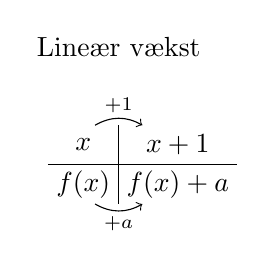
\begin{tikzpicture}
\node at (0,2) {Lineær vækst};
\foreach \i in {0}{
\draw (\i*0.9,0) -- (\i*0.9,1);
}
\draw (-0.9,0.5) -- (1.5,0.5);
\foreach \i in {0}{
\node at (\i*0.9+ 0.75,0.75) {$x+1$};
\node at (\i*0.9+0.75,0.25) {$f(x)+a$};
}
\node at (-0.45,0.75) {$x$};
\node at (-0.45,0.25) {$f(x)$};
\foreach \i in {0}{
\draw [->] (\i*0.9-0.3,1) to [out=30,in=150] (\i*0.9+0.3,1);
\node at (\i*0.9,1.25) {$\scriptstyle+1$};
\draw [->] (\i*0.9-0.3,-0) to [out=-30,in=-150] (\i*0.9+0.3,-0);
\node at (\i*0.9,-0.25) {$\scriptstyle+a$};
}
\end{tikzpicture}
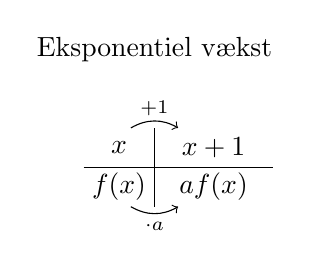
\begin{tikzpicture}
\node at (0,2) {Eksponentiel vækst};
\foreach \i in {0}{
\draw (\i*0.9,0) -- (\i*0.9,1);
}
\draw (-0.9,0.5) -- (1.5,0.5);
\foreach \i in {0}{
\node at (\i*0.9+ 0.75,0.75) {$x+1$};
\node at (\i*0.9+0.75,0.25) {$af(x)$};
}
\node at (-0.45,0.75) {$x$};
\node at (-0.45,0.25) {$f(x)$};
\foreach \i in {0}{
\draw [->] (\i*0.9-0.3,1) to [out=30,in=150] (\i*0.9+0.3,1);
\node at (\i*0.9,1.25) {$\scriptstyle+1$};
\draw [->] (\i*0.9-0.3,-0) to [out=-30,in=-150] (\i*0.9+0.3,-0);
\node at (\i*0.9,-0.25) {$\scriptstyle\cdot a$};
}
\end{tikzpicture}
\caption{Udvikling af lineær og eksponentiel vækst}
\label{fig:lineks}
\end{figure}
Vi kan desværre ikke få noget helt tilsvarende for potensvækst, da en øgning af $x$ med en vil give forskellige fremskrivninger af $f(x)$ alt efter hvad $x$ er. Vi kan derimod beskrive potensvækst ved følgende sætning.
\begin{setn}
Lad $f$ være en potensfunktion, altså 
\begin{align*}
f(x) = b\cdot a^x.
\end{align*}
Så vil en multiplikation af $x$ med en faktor $k$ tilsvare en stigning af $f(x)$ med en faktor $k^a$. Mere præcist gælder der, at 
\begin{align*}
f(k\cdot x) = k^a\cdot f(x).
\end{align*}
\end{setn}
\begin{proof}
Vi betragter 
\begin{align*}
f(k\cdot x) = b\cdot (k\cdot x)^a = b \cdot k^a \cdot x^a = k^a\cdot\underbrace{b\cdot x^a}_{=f(x)} = k^a \cdot f(x),
\end{align*}
hvilket beviser sætningen. 
\end{proof}
Det er værd at bemærke, at det at gange med $k$ tilsvarer at øge $x$ med $(k-1)\cdot 100 \%.$ Tilsvarende svarer multiplikation med $k^a$ til at øge $f(x)$ med $(k^a-1)\cdot 100\%$, så når vi øger $x$ med en hvis procent, så fås en tilsvarende procentvis øgning til $f(x)$. Derfor kaldes potensvækst til tider for $\%\%$-vækst. Lineær vækst kaldes til tider for $\Delta\Delta$-vækst og eksponentiel vækst kaldes til tider for $\Delta\%$-vækst. Fig. \ref{fig:potens}
\begin{figure}[H]
\centering
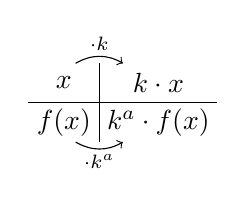
\begin{tikzpicture}
\foreach \i in {0}{
\draw (\i*0.9,0) -- (\i*0.9,1);
}
\draw (-0.9,0.5) -- (1.5,0.5);
\foreach \i in {0}{
\node at (\i*0.9+ 0.75,0.75) {$k\cdot x$};
\node at (\i*0.9+0.75,0.25) {$k^a \cdot f(x)$};
}
\node at (-0.45,0.75) {$x$};
\node at (-0.45,0.25) {$f(x)$};
\foreach \i in {0}{
\draw [->] (\i*0.9-0.3,1) to [out=30,in=150] (\i*0.9+0.3,1);
\node at (\i*0.9,1.25) {$\scriptstyle\cdot k$};
\draw [->] (\i*0.9-0.3,-0) to [out=-30,in=-150] (\i*0.9+0.3,-0);
\node at (\i*0.9,-0.25) {$\scriptstyle\cdot k^a$};
}
\end{tikzpicture}
\caption{Udvikling af potensvækst}
\label{fig:potens}
\end{figure}
\section*{Opgave 1}
\begin{enumerate}[label=\roman*)]
\item Potensfunktionen $f(x) = 2\cdot x^a$ går gennem punktet $(2,18)$. Brug dette til at bestemme $a$.
\item Potensfunktionen $f(x) = b\cdot x^1$ går gennem punktet $(3,3)$. Brug dette til at bestemme $b$.
\item Brug topunktsformlen til at bestemme den potensfunktion, der går gennem punkterne $(0.5,1)$, og $(1.5,1.5)$.
\item Brug topunktsformlen til at bestemme den potensfunktion, der går gennem punkterne $(1,1)$ og $(2,2)$.
\item Brug topunktsformlen til at bestemme den potensfunktion, der går gennem punkterne $(3,6)$ og $(4,5)$.
\item Brug topunktsformlen til at bestemme den potensfunktion, der går gennem punkterne $(2.11,13.5)$ og $(4.47,30.11)$.
\end{enumerate}
\section*{Opgave 2}
\begin{enumerate}
\item En potensfunktion er givet ved $f(x) = 1.5\cdot x^{1.5}$. Hvor meget stiger $f(x)$ med, hvis $x$ stiger med $10\%$? Hvad med $25\%$?
\item En potensfunktion er givet ved $f(x) = 10\cdot x^{-3}$. Hvor meget stiger $f(x)$ med, hvis $x$ stiger med $50\%$?
\item En potensfunktion er givet ved $f(x) = \sqrt{x}$. Hvor meget stiger $f(x)$ med, hvis $x$ stiger med $300\%$?
\end{enumerate}
\section*{Opgave 3}
Den effekt, det kræves at bevæge sig gennem luft med kan beskrives ved 
\begin{align*}
P(v) = K\cdot v^3,
\end{align*}
hvor $v$ beskriver hastigheden og $K$ er en konstant, der afhænger af en række forhold.
\begin{enumerate}[label=\roman*)]
\item Hvis vi øger hastigheden $v$ med $50\%$, hvor meget øges den effekt, der kræves for at bevæge sig gennem luften så med? 
\item Hvis vi øger vores effekt med $200\%$, hvor meget hurtigere kan vi så bevæge os gennem luften?
\end{enumerate}
\section*{Opgave 4}
Bremselængden for en bil kan beskrives ved $D$ givet ved
\begin{align*}
D(v) = k\cdot v^2.
\end{align*}
\begin{enumerate}[label=\roman*)]
\item Hvis vi øger hastigheden med $20\%$, hvor meget øges bremselængden $D$ så med?
\item Hvis vi vil sænke vores bremselængde med $50\%$, hvor meget skal vi så sænke vores hastighed med?
\end{enumerate}